%% =============================================================================
%% RESULTS CHAPTER -- standalone, Overleaf-ready single file
%% =============================================================================
%% Paste this file into a new Overleaf project (or compile locally with
%% pdflatex) -- no edits required. All section text and table data are
%% contained inline. Upload the 10 figure PDFs (see list below) to the
%% Overleaf project root or to a figures/ subfolder.
%%
%% Standalone preview numbers as Chapter 5 / sections 5.1-5.9 because the
%% preamble sets \setcounter{chapter}{4} before \chapter{Results}. To merge
%% into a host thesis where Results is already a chapter, delete everything
%% from line 1 down through \chapter{Results}\label{ch:results} and the
%% matching \end{document} at the bottom; paste the remaining body where the
%% Results chapter belongs in the host file.
%%
%% Sections (in document order):
%%   5.1 -- Evaluation setting and reporting protocol
%%   5.2 -- Statistical heterogeneity alone gives limited optimiser separation
%%   5.3 -- mu sensitivity: the proximal term helps only in a narrow range
%%   5.4 -- Li-style straggler asymmetry (CENTREPIECE)
%%   5.5 -- Learning-rate asymmetry reveals FedNova regime-dependence
%%   5.6 -- Rare-class collapse into mel-nevi
%%   5.7 -- Mechanism and robustness checks
%%   5.8 -- Integrated summary of findings
%%   5.9 -- Limitations
%%
%% Figure PDFs referenced (upload these to Overleaf):
%%   F_dataset_classes.pdf                          (Fig 5.1)
%%   F_statistical_heterogeneity_forest.pdf         (Fig 5.2 panel a)
%%   F_engineered_per_class.pdf                     (Fig 5.2 panel b)
%%   F_mu_sensitivity_outcome_and_convergence.pdf   (Fig 5.3)
%%   F_val_curves_extreme_gaps.pdf                  (Fig 5.4 panel A)
%%   F_l4_four_condition_per_class_grid.pdf         (Fig 5.4 panel B)
%%   F_asymmetric_lr_L4.pdf                         (Fig 5.5)
%%   F_heterogeneity_escalation.pdf                 (Fig 5.6)
%%   F_cross_experiment_per_class.pdf               (Fig 5.7)
%%   F_update_norms.pdf                             (Fig 5.8)
%% =============================================================================

\documentclass[11pt,a4paper]{report}

\usepackage[utf8]{inputenc}
\usepackage[T1]{fontenc}
\usepackage{graphicx}
\graphicspath{{mnist_dermnist/results/thesis_ready/figures/}{figures/}{./}}
\usepackage{booktabs}
\usepackage{amsmath, amssymb}
\usepackage{microtype}
\usepackage{hyperref}
\usepackage{caption}
\usepackage[margin=2.5cm]{geometry}

\title{Results Chapter Draft\\
\large DermaMNIST FedAvg vs FedProx vs FedNova}
\author{Barbara Koch}
\date{}

\begin{document}

\maketitle

%% =============================================================================
%% Chapter wrapper. \setcounter{chapter}{4} so the standalone preview numbers
%% sections 5.1, 5.2, ... matching the host thesis where this is Chapter 5.
%% =============================================================================
\setcounter{chapter}{4}
\chapter{Results}
\label{ch:results}




%%%%%%%%%%%%%%%%%%%%%%%%%%%%%%%%%%%%%%%%%%%%%%%%%%%%%%%%%%%%%%%%%%%%%%%%%%%%%%%
%% sec 5.1 -- Evaluation setting and reporting protocol
%%%%%%%%%%%%%%%%%%%%%%%%%%%%%%%%%%%%%%%%%%%%%%%%%%%%%%%%%%%%%%%%%%%%%%%%%%%%%%%

% =============================================================================
% Results sec 5.1 -- Evaluation setting and reporting protocol
% Compressed. Definitional, not interpretive. Target ~250 words.
% Verified facts: class supports (66.9% / 1.1% / 1.4%); test counts;
% RARE_IDX = {dermato, melanoma, vascular} (canonical).
% =============================================================================

\section{Evaluation setting and reporting protocol}
\label{sec:eval-setting}

DermaMNIST is severely class-imbalanced: mel-nevi occupies $66.9\,\%$ of
the training set while dermato and vascular together account for $2.5\,\%$,
with test supports of $1341/2005$ images for mel-nevi versus $23$ for
dermato and $29$ for vascular (Figure~\ref{fig:dataset-classes}). Raw
accuracy would saturate at the mel-nevi prevalence floor, so the primary
metric throughout is test macro-F1 at the best-validation checkpoint, with
per-class F1, confusion-matrix diagonal entries, and rare-class F1 as
secondary diagnostics. Rare-class F1 uses the canonical index set
$\mathrm{RARE\_IDX} = \{\text{dermato}, \text{melanoma}, \text{vascular}\}$;
the $0.265$ value from earlier drafts excluded melanoma and is not used.

Three seed tiers are reported distinctly. Headline comparisons use $n = 10$
paired seeds with the within-pair sign count and Wilcoxon signed-rank where
applicable. Mechanism and asymmetry probes use $n = 3$ as directional only;
no significance test is applied at this sample size. Single-seed pilots
(notably the heterogeneity ladder) are labelled explicitly and are not used
to derive headline numbers.

Two runtimes are used: a pure-PyTorch reference loop and a Flower
simulation. Their estimates diverge on the engineered partition
(\S\,\ref{sec:statistical-heterogeneity}); the chapter takes the Flower
paired replication as the central headline because it carries
\texttt{git\_commit} and per-round \texttt{client\_update\_norms} provenance
that the pure-PyTorch loop does not.

Table~\ref{tab:reporting-protocol} summarises these conventions; subsequent
sections cite them only by reference.


% =============================================================================
% Table 5.1
% =============================================================================

\begin{table}[h]
\centering
\small
\caption{Reporting protocol and metric hierarchy. Applied uniformly across
\S\S\,5.2--5.9.}
\label{tab:reporting-protocol}
\begin{tabular}{p{0.20\linewidth} p{0.32\linewidth} p{0.40\linewidth}}
\hline
Component               & Choice                                       & Reason \\
\hline
Primary metric          & Test macro-F1 at best-val checkpoint         & Class-imbalanced; accuracy saturates at majority floor \\
Secondary metrics       & Per-class F1, confusion-matrix diagonal, rare-F1 & Surface per-class failure that macro can mask \\
Rare-class definition   & $\{\text{dermato}, \text{melanoma}, \text{vascular}\}$ & Low support + high clinical priority (melanoma is mid-support but high-stakes) \\
$n = 10$ protocol       & Paired sign count + Wilcoxon where applicable & Headline statistical-heterogeneity comparisons \\
$n = 3$ protocol        & Directional only; no significance test       & Mechanism probes; power insufficient for $p$-values \\
$n = 1$ protocol        & Labelled ``pilot''; no headline use          & Heterogeneity ladder; single-class seed events possible \\
Runtimes                & Flower (central), pure-PyTorch (corroboration) & Flower carries full git+update-norm provenance \\
\hline
\end{tabular}
\end{table}


% =============================================================================
% Figure 5.1
% =============================================================================

\begin{figure}[h]
\centering
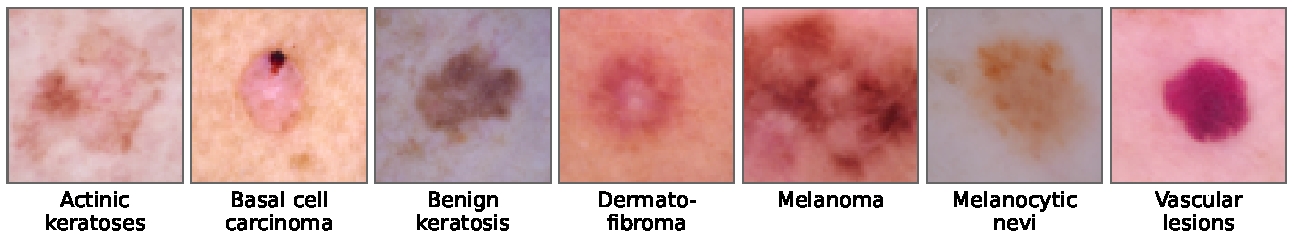
\includegraphics[width=0.7\textwidth]{F_dataset_classes.pdf}
\caption{DermaMNIST class distribution. Mel-nevi dominates at $66.9\,\%$ of
the training set; dermato ($1.1\,\%$), vascular ($1.4\,\%$), and melanoma
(${\approx}11\,\%$) define the rare-class set used throughout the chapter.}
\label{fig:dataset-classes}
\end{figure}



%%%%%%%%%%%%%%%%%%%%%%%%%%%%%%%%%%%%%%%%%%%%%%%%%%%%%%%%%%%%%%%%%%%%%%%%%%%%%%%
%% sec 5.2 -- Statistical heterogeneity alone gives limited optimiser separation
%%%%%%%%%%%%%%%%%%%%%%%%%%%%%%%%%%%%%%%%%%%%%%%%%%%%%%%%%%%%%%%%%%%%%%%%%%%%%%%

% =============================================================================
% Results sec 5.2 -- Statistical heterogeneity alone gives limited separation
% Compressed version. All numerics verified against VERIFICATION_SHEET.txt.
% Target ~500 words.
% =============================================================================

\section{Statistical heterogeneity alone gives limited optimiser separation}
\label{sec:statistical-heterogeneity}

Under an IID partition (Flower, $n=10$ paired seeds), FedAvg and FedProx
differ by $\Delta = -0.007$ macro-F1 (FA $0.585$, FP $0.578$, FN $0.577$) ---
within seed noise. We treat this as a negative control: statistical
heterogeneity is a necessary condition for any FedAvg--FedProx gap on this
benchmark.

On the engineered balanced-paired seven-client partition we report three
estimates ($n=10$ paired seeds each): Flower paired $\Delta = +0.007$ (7/10
paired wins, full \texttt{git\_commit} and \texttt{client\_update\_norms}
provenance), Flower $\mu$-sweep peak at $\mu = 0.01$ $\Delta = +0.013$ (full
provenance, $\mu$ characterisation in \S\,\ref{sec:mu-sensitivity}), and
pure-PyTorch reference $\Delta = +0.027$ (9/10 wins, no \texttt{git\_commit},
no companion update-norm logs). All three measure the same partition through
slightly different code paths; they agree on sign and bracket the magnitude
at $0.01$--$0.03$. The Flower paired $\Delta = +0.007$ is the central
headline; the pure-PyTorch number is cross-runtime corroboration.

The pure-PyTorch $+0.027$ is concentrated in two classes: melanoma
contributes $+0.114$ per-class F1 (61\,\% share of the macro-F1 advantage)
and actinic keratoses $+0.067$ (36\,\%); the other five classes contribute
the residual 3\,\% (all $|\Delta| \leq 0.013$), and mel-nevi is invariant at
$+0.002$. Figure~\ref{fig:engineered-per-class} renders the per-class
validation trajectories under the engineered partition ($n=10$ paired
seeds, $\pm 1$ SEM bands): the melanoma and actinic panels show non-
overlapping FedAvg vs FedProx bands by mid-training, while the other five
classes (including mel-nevi) overlap throughout 150 rounds. The gain
reflects rebalancing of two minority classes, not a uniform optimiser
improvement.

Three other partitions replicate the small-magnitude finding: Dirichlet
$\alpha = 0.1$ $\Delta = +0.008$ ($n=10$), specialist 1-of-7 $\Delta = +0.008$
($n=10$), multi-seed node-pinned L4 $\Delta = +0.005$ ($n=3$; per-seed
$\{+0.013, +0.019, -0.016\}$). The single-seed heterogeneity-ladder pilot
at L4 gives $\Delta = -0.030$, but its $-0.030$ deficit is driven entirely
by vascular F1 dropping by $-0.220$ (FA $0.702$ $\rightarrow$ FP $0.482$);
all six other classes are within $|\Delta| \leq 0.034$. The aggregate is one
rare-class outcome on one seed, and the $n=3$ node-pinned promotion
($\Delta = +0.005$) averages it out. All Dirichlet aggregates above use
regenerated raw-JSON summaries; the previously-committed analysis CSVs were
stale and showed a spurious seed-8675309 catastrophic FedProx failure that
the regenerated data do not support.

On the engineered partition, FedProx reduces test-macro-F1 SD from $0.025$
to $0.014$ ($-45\,\%$), reaches validation macro-F1 $= 0.40$ in $9.8$ vs
$12.7$ rounds ($1.3\times$ speed-up), and shows a paired mid-training peak
$\Delta = +0.094$ at round 50 that closes to $+0.007$ by round 150. These
trajectory characteristics are documented for the engineered partition only.

Statistical heterogeneity alone produces small, runtime-sensitive separation
(Table~\ref{tab:stat-het-headline}, Figure~\ref{fig:stat-het-forest}). The
next question is whether the proximal coefficient $\mu$ itself explains when
FedProx helps.


% =============================================================================
% Table 5.2 placeholder
% =============================================================================

\begin{table}[h]
\centering
\caption{Statistical heterogeneity and runtime sensitivity. Six cells:
IID, the engineered partition through two runtimes plus the $\mu$-peak,
Dirichlet $\alpha=0.1$, specialist 1-of-7, and the multi-seed node-pinned
L4 control. Dirichlet, specialist, and IID values from regenerated raw-JSON
aggregates.}
\label{tab:stat-het-headline}
\resizebox{\textwidth}{!}{%
\begin{tabular}{lccccccl}
\hline
Setting              & Runtime       & Clients & $n$ & FedAvg              & FedProx             & $\Delta$ & Note \\
\hline
IID                  & Flower        & 7       & 10  & $0.585 \pm 0.020$   & $0.578 \pm 0.020$   & $-0.007$ & negative control \\
Engineered (pure)    & pure-PyTorch  & 7       & 10  & $0.481 \pm 0.025$   & $0.508 \pm 0.014$   & $+0.027$ & 9/10 wins; partial provenance \\
Engineered (Flower)  & Flower        & 7       & 10  & $0.496$             & $0.503$             & $+0.007$ & 7/10 wins; \textbf{central} \\
Dirichlet $\alpha=0.1$ & Flower      & 7       & 10  & $0.480 \pm 0.036$   & $0.488 \pm 0.034$   & $+0.008$ & regenerated raw-JSON \\
Specialist 1-of-7    & Flower        & 7       & 10  & $0.437 \pm 0.024$   & $0.445 \pm 0.017$   & $+0.008$ & --- \\
Node-pinned L4       & Flower        & 2       & 3   & $0.492 \pm 0.019$   & $0.497 \pm 0.022$   & $+0.005$ & multi-seed L4 control \\
\hline
\end{tabular}%
}
\end{table}


% =============================================================================
% Figure 5.2 placeholder
% =============================================================================

\begin{figure}[h]
\centering
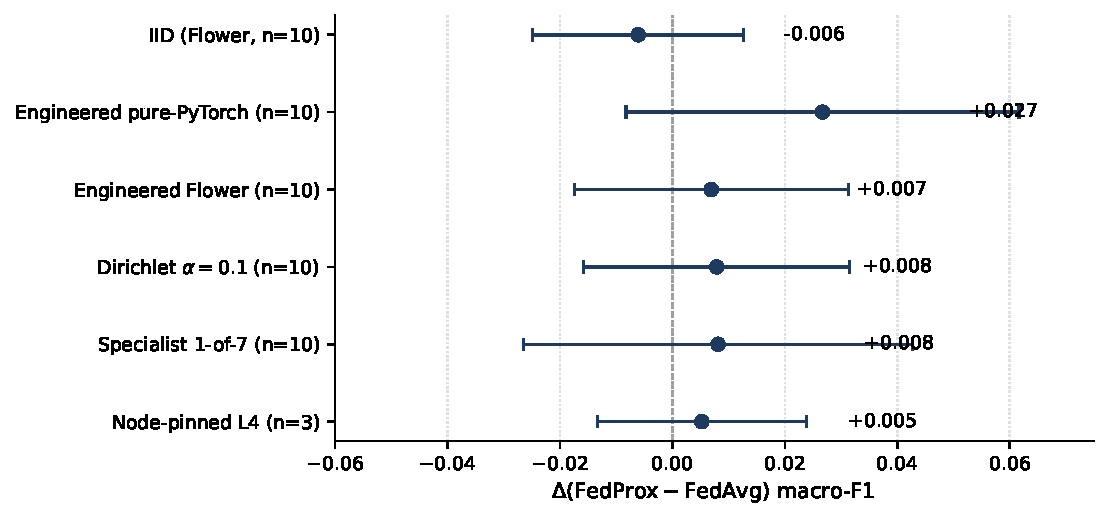
\includegraphics[width=0.85\textwidth]{F_statistical_heterogeneity_forest.pdf}
\caption{Forest plot of $\Delta(\textrm{FedProx} - \textrm{FedAvg})$ macro-F1
across the six settings in Table~\ref{tab:stat-het-headline}. Whiskers show
$\pm 1$ sample SD across paired seeds; dashed line at $\Delta = 0$ marks no
separation. The IID negative control sits at the left; the five partitioned
settings cluster between $+0.005$ and $+0.027$.}
\label{fig:stat-het-forest}
\end{figure}


% =============================================================================
% Figure 5.2(b) -- engineered partition per-class trajectories
% =============================================================================

\begin{figure}[h]
\centering

\includegraphics[width=\textwidth]{F_engineered_per_class.pdf}
\caption{Per-class validation F1 trajectories on the engineered partition,
$n = 10$ paired seeds (FedAvg vs FedProx, mean $\pm 1$ SEM bands).
Two-by-four grid (seven classes plus legend). Melanoma and actinic-keratoses
panels show non-overlapping FedAvg/FedProx bands by mid-training --- the
two classes that carry the pure-PyTorch $+0.027$ macro-F1 advantage
($+0.114$ and $+0.067$ per-class F1, $61\,\%$ and $36\,\%$ of the share
respectively). The other five classes show overlapping bands throughout
150 rounds, including the dominant mel-nevi panel which is invariant near
its prevalence saturation.}
\label{fig:engineered-per-class}
\end{figure}



%%%%%%%%%%%%%%%%%%%%%%%%%%%%%%%%%%%%%%%%%%%%%%%%%%%%%%%%%%%%%%%%%%%%%%%%%%%%%%%
%% sec 5.3 -- mu sensitivity: the proximal term helps only in a narrow range
%%%%%%%%%%%%%%%%%%%%%%%%%%%%%%%%%%%%%%%%%%%%%%%%%%%%%%%%%%%%%%%%%%%%%%%%%%%%%%%

% =============================================================================
% Results sec 5.3 -- mu sensitivity
% Compressed version. Target ~300 words.
% =============================================================================

\section{$\mu$ sensitivity: the proximal term helps only in a narrow range}
\label{sec:mu-sensitivity}

A five-cell sweep of $\mu \in \{0.001, 0.01, 0.1, 1.0\}$ against the FedAvg
baseline ($\mu = 0$) on the engineered partition ($n=10$ paired seeds per
cell) traces a clear inverted-$U$ (Table~\ref{tab:mu-sweep},
Figure~\ref{fig:mu-inverted-u}): peak near $\mu = 0.01$, dropping below
baseline by $\mu = 0.1$ and catastrophic at $\mu = 1.0$.

FedAvg gives $0.493 \pm 0.020$. FedProx at $\mu = 0.001$ reaches
$0.504 \pm 0.021$ ($\Delta = +0.011$, 6/10 paired wins); at $\mu = 0.01$ it
peaks at $0.506 \pm 0.017$ ($\Delta = +0.013$, 6/10 wins) --- numerically
indistinguishable from the $\mu = 0.001$ cell. At $\mu = 0.1$ the mean falls
to $0.479 \pm 0.017$ ($\Delta = -0.014$, 2/10 wins); at $\mu = 1.0$ it
collapses to $0.419 \pm 0.013$ ($\Delta = -0.074$, 0/10 wins --- every seed
loses). The $0.09$ macro-F1 spread between best and worst $\mu$ is an order
of magnitude larger than any partition-level $\Delta$ in
\S\,\ref{sec:statistical-heterogeneity}.

The $\mu$-sweep peak $\Delta = +0.013$ exceeds the
\S\,\ref{sec:statistical-heterogeneity} Flower paired $\Delta = +0.007$
because the sweep selects best-of-five on the same seeds; the two estimates
bracket the same small effect at $+0.005$ to $+0.015$.

The practical region of useful $\mu$ on this benchmark is a single decade
around $0.01$. The expectation that larger $\mu$ should be preferred under
stronger statistical heterogeneity is not supported here --- a benchmark
observation, not a refutation of the underlying analysis.

Table~\ref{tab:mu-per-class} breaks down the $\mu = 1.0$ catastrophic cell
per class. The deficit is concentrated in the rare and minority classes
(dermato $-0.101$, vascular $-0.113$, actinic $-0.124$) while the dominant
mel-nevi is essentially invariant ($-0.017$). The same rare-class
sensitivity that drives the catastrophic large-$\mu$ regime is the
clinical failure mode characterised in
\S\,\ref{sec:rare-class-collapse}; large-$\mu$ FedProx fails in the same
shape as the dropped-stragglers and asymmetric-LR cells, only via a
different mechanism (over-regularisation rather than under-aggregation).
Because $\mu$ alone is sensitive and at larger values harmful, the much
larger FedProx gains under straggler protocols
(\S\,\ref{sec:li-straggler}) cannot be attributed to the proximal
coefficient itself.


% =============================================================================
% Table 5.3 placeholder
% =============================================================================

\begin{table}[h]
\centering
\caption{$\mu$ sensitivity on the engineered partition, $n=10$ paired
seeds per cell. ``Wins'' is paired comparisons where FedProx exceeds
FedAvg on the matched seed.}
\label{tab:mu-sweep}
\begin{tabular}{ccccl}
\hline
$\mu$    & macro-F1 (mean $\pm$ SD) & $\Delta$ vs FedAvg & Wins / 10 & Interpretation \\
\hline
$0$      & $0.493 \pm 0.020$        & ---               & ---       & FedAvg baseline                \\
$0.001$  & $0.504 \pm 0.021$        & $+0.011$          & 6         & near peak                      \\
$0.01$   & $\mathbf{0.506 \pm 0.017}$ & $\mathbf{+0.013}$ & 6       & \textbf{peak}                  \\
$0.1$    & $0.479 \pm 0.017$        & $-0.014$          & 2         & below baseline                 \\
$1.0$    & $0.419 \pm 0.013$        & $-0.074$          & 0         & catastrophic                   \\
\hline
\end{tabular}
\end{table}


% =============================================================================
% Figure 5.3 placeholder
% =============================================================================

\begin{figure}[h]
\centering
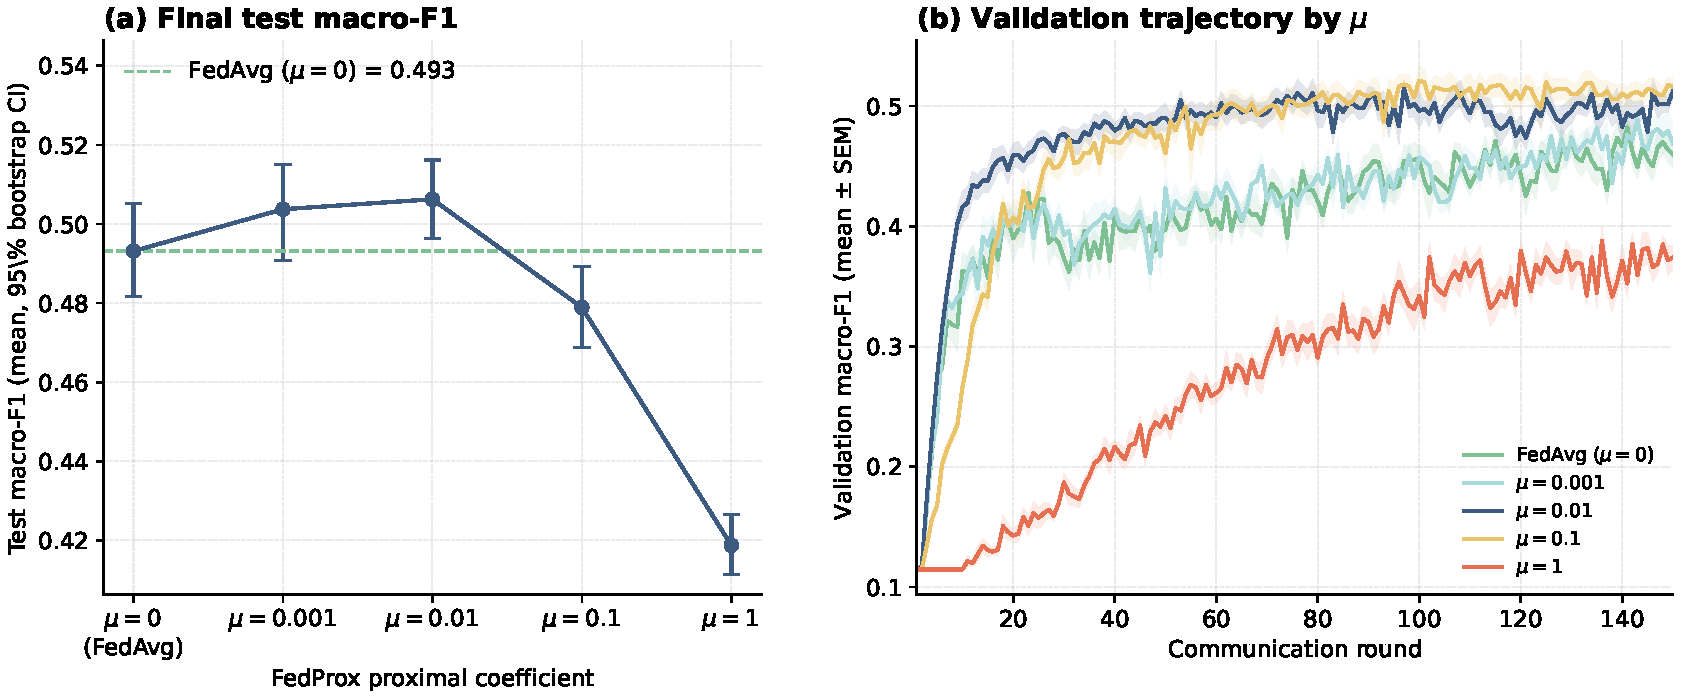
\includegraphics[width=0.85\textwidth]{F_mu_sensitivity_outcome_and_convergence.pdf}
\caption{Inverted-$U$ $\mu$ sensitivity curve on the engineered partition
($n=10$ per cell). $x$-axis: $\mu$ on $\log_{10}$ scale across
$\{0.001, 0.01, 0.1, 1.0\}$, FedAvg baseline as dashed reference line at
$0.493$. $y$-axis: test macro-F1 with $\pm 1$ SD whiskers.}
\label{fig:mu-inverted-u}
\end{figure}


% =============================================================================
% Table 5.3b -- per-class mu sensitivity (engineered partition)
% =============================================================================

\begin{table}[h]
\centering
\small
\caption{Per-class validation F1 mean across the $\mu$ sweep on the
engineered partition, $n = 10$ paired seeds per cell. SDs across seeds
range $0.003$ (mel-nevi) to $0.113$ (rare classes). ``$\Delta$ at $\mu=1.0$''
is the absolute per-class F1 deficit at the catastrophic cell relative to
the FedAvg baseline ($\mu = 0$). The deficit concentrates in rare and
minority classes; the dominant mel-nevi class is essentially invariant.
Source: \texttt{mu\_sensitivity\_flower/}.}
\label{tab:mu-per-class}
\begin{tabular}{lcccccc}
\hline
Class       & $\mu = 0$ & $\mu = 0.001$ & $\mu = 0.01$ & $\mu = 0.1$ & $\mu = 1.0$ & $\Delta$ at $\mu = 1.0$ \\
\hline
actinic     & $0.475$   & $0.470$       & $0.489$      & $0.434$     & $0.351$     & $-0.124$ \\
basal       & $0.497$   & $0.513$       & $0.497$      & $0.405$     & $0.438$     & $-0.060$ \\
b-kerat     & $0.405$   & $0.400$       & $0.423$      & $0.416$     & $0.328$     & $-0.077$ \\
dermato     & $0.259$   & $0.287$       & $0.283$      & $0.279$     & $0.158$     & $\mathbf{-0.101}$ \\
melanoma    & $0.244$   & $0.258$       & $0.304$      & $0.287$     & $0.216$     & $-0.028$ \\
mel-nevi    & $0.884$   & $0.885$       & $0.886$      & $0.886$     & $0.867$     & $-0.017$ \\
vascular    & $0.687$   & $0.713$       & $0.661$      & $0.646$     & $0.574$     & $\mathbf{-0.113}$ \\
\hline
\end{tabular}
\end{table}



%%%%%%%%%%%%%%%%%%%%%%%%%%%%%%%%%%%%%%%%%%%%%%%%%%%%%%%%%%%%%%%%%%%%%%%%%%%%%%%
%% sec 5.4 -- Li-style straggler asymmetry (CENTREPIECE)
%%%%%%%%%%%%%%%%%%%%%%%%%%%%%%%%%%%%%%%%%%%%%%%%%%%%%%%%%%%%%%%%%%%%%%%%%%%%%%%

% =============================================================================
% Results sec 5.4 -- Centrepiece
% Compressed version. Target ~720 words (centrepiece stays substantive).
% =============================================================================

\section{Under Li-style straggler asymmetry, FedProx's advantage is mediated
mainly by $\gamma$-inexact partial-update handling}
\label{sec:li-straggler}

The straggler-regime FedProx advantage requires both statistical and system
heterogeneity: removing statistical heterogeneity from the straggler
protocol does not shrink the gain, it reverses it. Under
\texttt{system\_het\_iid\_random} (IID partition, $n=10$), $\Delta = -0.013$
macro-F1; under the identical straggler schedule on the L4 partition
(\texttt{system\_het\_random}, $n=10$), $\Delta = +0.017$. Stragglers alone
are neutral; label imbalance alone gives the small effects in
\S\,\ref{sec:statistical-heterogeneity}; their combination opens a
$3$-percentage-point window in which optimiser choice matters, and
motivates the four-condition decomposition below.

We decompose the gap into four matched cells at L4, $n=3$
(Table~\ref{tab:li-decomp-l4}). \emph{FedAvg, no straggler} establishes the
no-system-heterogeneity baseline. \emph{FedAvg + drop} adds the straggler
protocol but discards stragglers' partial updates. \emph{FedProx + drop}
adds the proximal term while holding the drop policy fixed, isolating the
proximal contribution alone. \emph{FedProx + $\gamma$-inexact} replaces the
drop policy with $\gamma$-inexact partial-update acceptance, isolating the
partial-update mechanism on top of the proximal term. All remaining
hyperparameters are held fixed.

L4 cells give FedAvg-no-straggler $0.485 \pm 0.028$, FA+drop
$0.364 \pm 0.009$, FP+drop $0.368 \pm 0.005$, FP+$\gamma$-inex
$0.479 \pm 0.010$. The total gap over FA+drop is $+0.115$, decomposing as
proximal-only $+0.004$ (FP+drop $-$ FA+drop) and $\gamma$-inexact $+0.111$
(FP+$\gamma$-inex $-$ FP+drop). Within the FedProx protocol, approximately
$96\,\%$ of the straggler-regime gain over FedAvg+drop is mediated by
partial-update acceptance rather than by the proximal regulariser. The
decomposition does not include an FedAvg+$\gamma$-inex cell, so the
attribution is to the FedProx+$\gamma$-inex protocol rather than to
$\gamma$-inex as a standalone mechanism.
Figure~\ref{fig:val-curves-extreme-gaps}~(A) confirms this at the aggregate
level: the FA+drop and FP+drop validation trajectories overlap throughout all
150 rounds, while FP+$\gamma$-inex diverges upward around round 30 and
stabilises near $0.48$. Under matched drop-handling the proximal term
changes neither convergence rate nor asymptote; the partial-update accept
policy does both. Figure~\ref{fig:l4-per-class-grid} resolves this per
class: mel-nevi saturates at $\approx 0.89$ under all four conditions and is
invariant; the three rare classes (dermato, melanoma, vascular) flatline at
zero under FedAvg+drop and FedProx+drop, recover partially under
FedAvg-no-straggler ($\overline{\text{rare-F1}} = 0.17$), and recover
furthest under FedProx+$\gamma$-inexact
($\overline{\text{rare-F1}} = 0.25$, with melanoma reaching $0.36$). The
aggregate $\gamma$-inexact gain is localised to the rare-class learning
trajectory, not to the dominant class.

A stress test (L4, full straggler schedule, batch size 10,
accept-partial-updates, $n=3$) magnifies the same ordering. FedAvg+drop's
validation trajectory flatlines at each seed's round-1 value for all 150
rounds (s42: $0.114$, s123: $0.115$, s456: $0.030$); the best-validation
checkpoint is selected at round 1 for every seed --- the untrained
initialisation beats every trained checkpoint. Across seeds the mean test
macro-F1 is $0.087 \pm 0.049$. FedProx $\mu = 1.0$ recovers to $0.365 \pm 0.023$;
FedProx $\mu = 0.01$ reaches $0.491 \pm 0.003$, matching its four-condition
value. The $\approx +0.40$ gap demonstrates the same ordering at larger
magnitude but is not a clean decomposition: multiple hyperparameters change
between cells. The causal claim rests on Table~\ref{tab:li-decomp-l4};
perfect-storm only shows the mechanism survives stress severe enough to
make the trained model lose to its own initialisation.

To test whether the mechanism is generic or requires informationally unique
class signal at the dropped client, we ran the identical four-condition
design at L1 --- a quantity-only heterogeneity partition (86/14 sample
split, identical label distributions across clients, JS divergence
$\approx 0$). The L1 cells (Table~\ref{tab:li-decomp-l1}, $n=3$) are
essentially flat: FA-no-strag $0.601 \pm 0.010$, FA+drop $0.599 \pm 0.006$,
FP+drop $0.593 \pm 0.022$, FP+$\gamma$-inex $0.605 \pm 0.009$.
Proximal-only $-0.006$, $\gamma$-inexact $+0.012$, drop-cost $-0.001$ ---
versus $+0.111$ and $-0.121$ at L4. The $\gamma$-inexact contribution
shrinks by an order of magnitude, and drop-handling stops costing anything
measurable. $\gamma$-inexact partial-update acceptance has nothing to
rescue when the dropped client carries no class signal the other client
lacks: the mechanism is not generic drift-control but operates only when
statistical heterogeneity makes the dropped client's partial updates
informationally irreplaceable. The Table~\ref{tab:li-decomp-l4} vs
Table~\ref{tab:li-decomp-l1} contrast is the strongest single piece of
evidence for this interpretation in the chapter.

The straggler experiments isolate one axis of system asymmetry.
\S\,\ref{sec:lr-asymmetry} asks whether persistent learning-rate imbalance
--- a different axis --- changes the optimiser ranking.


% =============================================================================
% Tables
% =============================================================================

\begin{table}[h]
\centering
\caption{Li-style four-condition decomposition at the L4 partition,
$n=3$ matched seeds (42, 123, 456). Total gap over FA+drop $= +0.115$;
proximal-only contribution $+0.004$; $\gamma$-inexact contribution $+0.111$.
Source: \texttt{li2020\_asymmetric\_L4/analysis/li2020\_asymmetric\_L4\_summary.csv}.}
\label{tab:li-decomp-l4}
\begin{tabular}{lccccc}
\hline
Condition & Straggler? & Partial-update & Proximal? & macro-F1 & $\Delta$ vs FA+drop \\
\hline
FedAvg, no straggler        & no  & ---                  & no  & $0.485 \pm 0.028$ & $+0.121$ \\
FedAvg + drop               & yes & dropped              & no  & $0.364 \pm 0.009$ & ---      \\
FedProx + drop              & yes & dropped              & yes & $0.368 \pm 0.005$ & $+0.004$ \\
FedProx + $\gamma$-inexact  & yes & accepted ($\gamma$)  & yes & $0.479 \pm 0.010$ & $+0.115$ \\
\hline
\end{tabular}
\end{table}

\begin{table}[h]
\centering
\caption{Cross-partition control: same four-condition design at L1
(quantity-only heterogeneity, JS $\approx 0$, $n=3$). Schema matches
Table~\ref{tab:li-decomp-l4}. Decomposition: proximal-only $-0.006$,
$\gamma$-inexact $+0.012$, drop-cost $-0.001$ --- versus $+0.111$ and
$-0.121$ at L4. Source: \texttt{li2020\_asymmetric\_L1/}.}
\label{tab:li-decomp-l1}
\begin{tabular}{lccccc}
\hline
Condition & Straggler? & Partial-update & Proximal? & macro-F1 & $\Delta$ vs FA+drop \\
\hline
FedAvg, no straggler        & no  & ---                  & no  & $0.601 \pm 0.010$ & $+0.002$ \\
FedAvg + drop               & yes & dropped              & no  & $0.599 \pm 0.006$ & ---      \\
FedProx + drop              & yes & dropped              & yes & $0.593 \pm 0.022$ & $-0.006$ \\
FedProx + $\gamma$-inexact  & yes & accepted ($\gamma$)  & yes & $0.605 \pm 0.009$ & $+0.006$ \\
\hline
\end{tabular}
\end{table}


% =============================================================================
% Figure 5.4 placeholder
% =============================================================================

\begin{figure}[h]
\centering
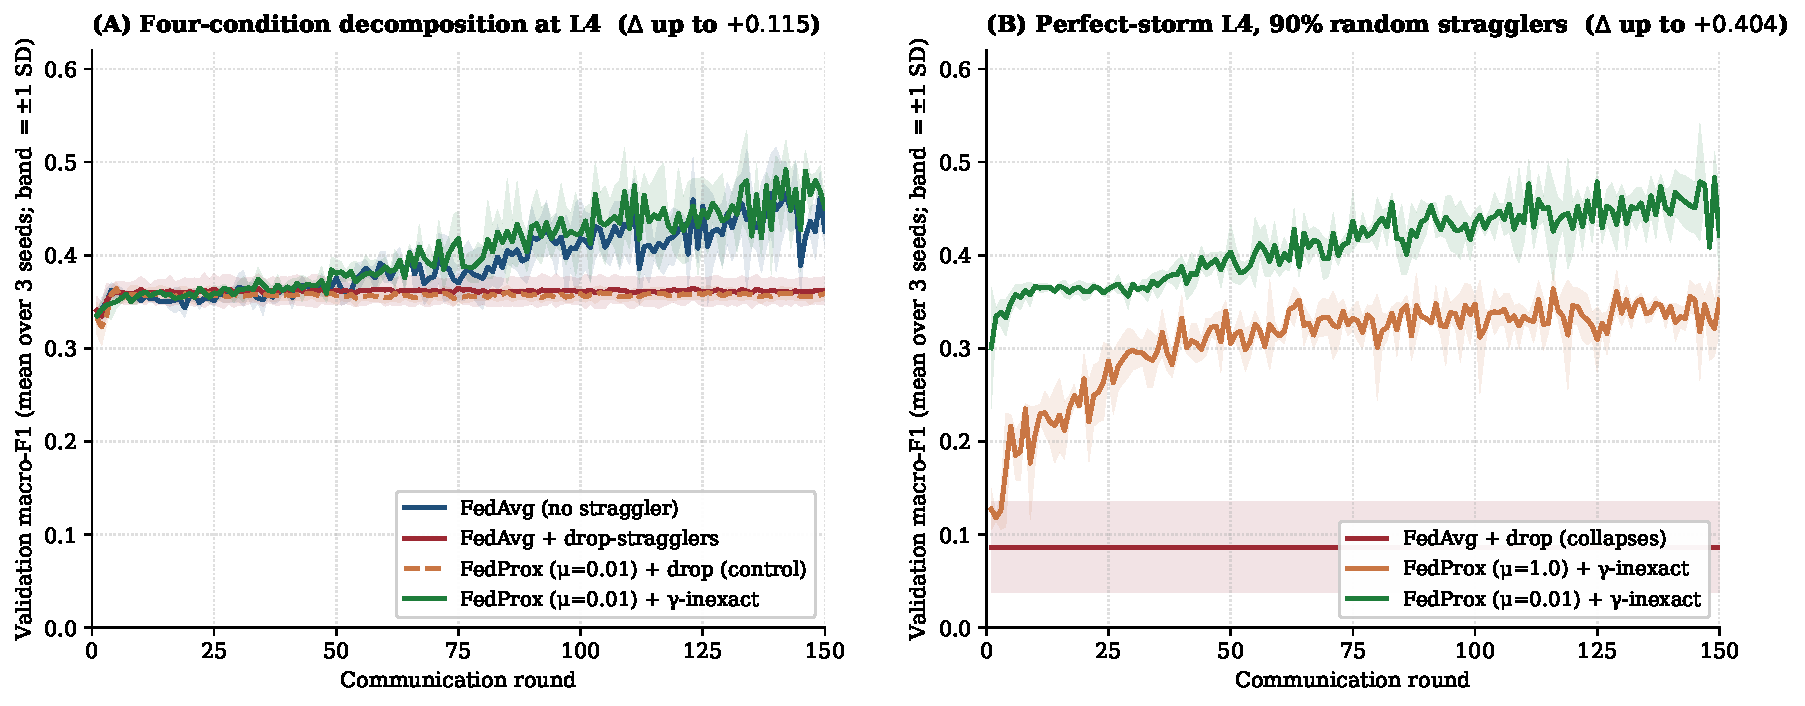
\includegraphics[width=0.85\textwidth]{F_val_curves_extreme_gaps.pdf}
\caption{Four-condition validation trajectories at L4, mean over $n=3$ seeds
(Panel A). FedAvg+drop and FedProx+drop overlap throughout 150 rounds,
isolating the proximal term as inactive under matched drop-handling.
FedProx+$\gamma$-inexact diverges upward around round 30 and stabilises
near $0.48$. Panel B (perfect-storm trajectories) is in Appendix~C.}
\label{fig:val-curves-extreme-gaps}
\end{figure}


% =============================================================================
% Figure 5.4(b) -- per-class trajectory grid (this session)
% =============================================================================

\begin{figure}[h]
\centering
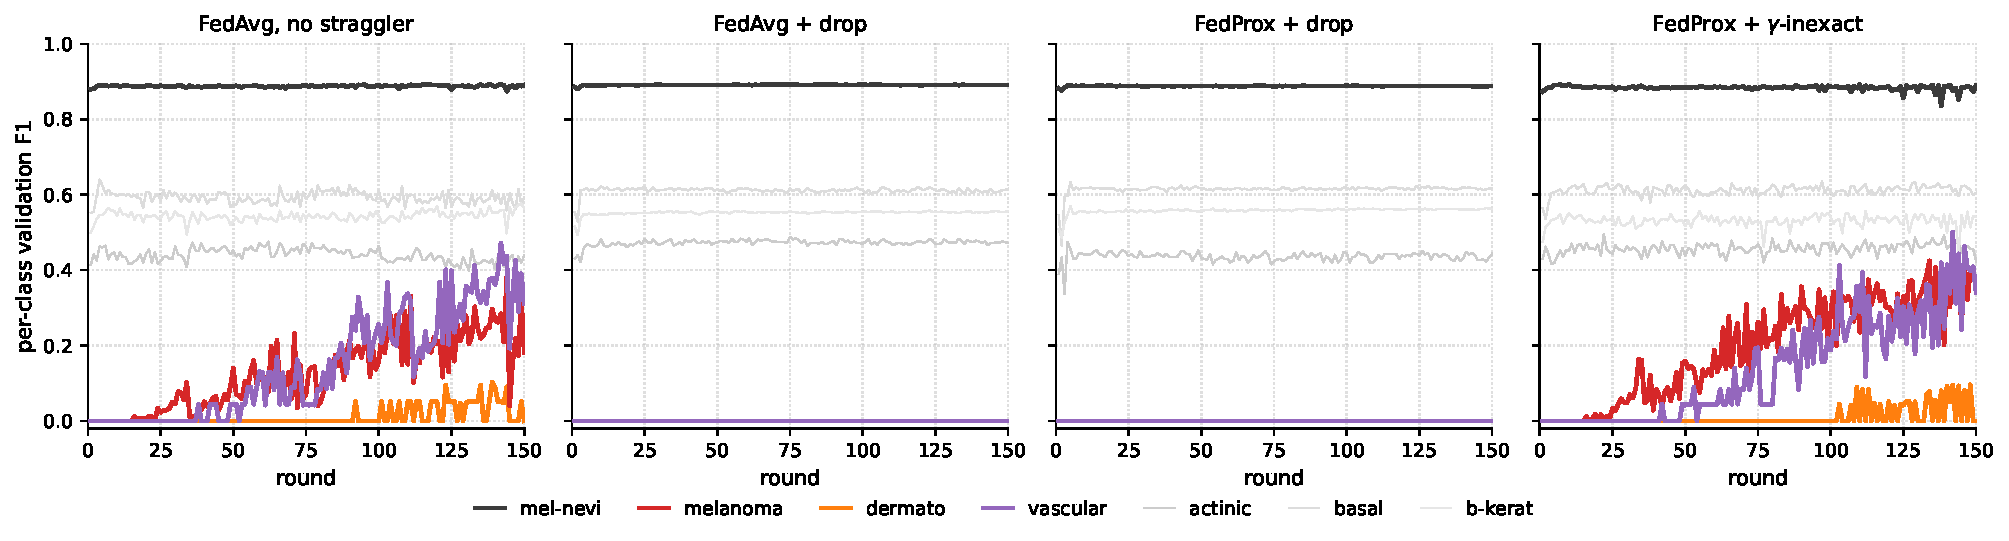
\includegraphics[width=\textwidth]{F_l4_four_condition_per_class_grid.pdf}
\caption{Per-class validation F1 trajectories under each of the four
conditions at L4, mean across $n = 3$ seeds. Mel-nevi (dark grey) is
invariant near $0.89$ across all conditions; the three rare classes ---
melanoma (red), dermato (orange), vascular (purple) --- flatline at zero
under FedAvg+drop and FedProx+drop and recover only under
FedProx+$\gamma$-inexact (melanoma to $\approx 0.36$, rare-F1 mean $0.25$).
The three common classes (light greys: actinic, basal, b-kerat) are shown
muted. The $\gamma$-inexact mechanism is localised to the rare-class
learning trajectory.}
\label{fig:l4-per-class-grid}
\end{figure}



%%%%%%%%%%%%%%%%%%%%%%%%%%%%%%%%%%%%%%%%%%%%%%%%%%%%%%%%%%%%%%%%%%%%%%%%%%%%%%%
%% sec 5.5 -- Learning-rate asymmetry reveals FedNova regime-dependence
%%%%%%%%%%%%%%%%%%%%%%%%%%%%%%%%%%%%%%%%%%%%%%%%%%%%%%%%%%%%%%%%%%%%%%%%%%%%%%%

% =============================================================================
% Results sec 5.5 -- Learning-rate asymmetry, FedNova regime-dependence
% Compressed version. Target ~560 words.
% =============================================================================

\section{Learning-rate asymmetry reveals FedNova regime-dependence}
\label{sec:lr-asymmetry}

On L4, Client 0 (the dominant client, $\approx 90\,\%$ of training samples)
keeps $\textrm{lr} = 0.01$ while Client 1 (rare classes) takes
$\textrm{lr} \in \{0.01, 0.005, 0.002, 0.001, 0.0005, 0.0002\}$, giving six
asymmetry ratios from 1:1 to 50:1 across FedAvg, FedProx, and FedNova
($n=3$ matched seeds per cell, 54 runs total). Test macro-F1 across the
envelope splits the three optimisers cleanly:

\begin{center}
\begin{tabular}{cccc|c}
\hline
Ratio & FedAvg & FedProx & FedNova & $\Delta_{\mathrm{FN-FA}}$ \\
\hline
 1:1  & $0.457$ & $0.491$ & $\mathbf{0.509}$ & $+0.052$ \\
 2:1  & $0.425$ & $0.462$ & $\mathbf{0.526}$ & $+0.101$ \\
 5:1  & $0.375$ & $0.392$ & $\mathbf{0.504}$ & $+0.129$ \\
10:1  & $0.369$ & $0.369$ & $\mathbf{0.501}$ & $+0.132$ \\
20:1  & $0.367$ & $0.372$ & $\mathbf{0.486}$ & $+0.119$ \\
50:1  & $0.367$ & $0.367$ & $\mathbf{0.498}$ & $\mathbf{+0.131}$ \\
\hline
\end{tabular}
\end{center}

FedAvg and FedProx drop $\approx 0.10$ macro-F1 between 1:1 and 5:1 and then
plateau at the rare-class floor near $0.367$; FedNova stays in the
$0.486$--$0.526$ band across the entire envelope ($|\Delta$ vs its own 1:1
baseline$|$ $\leq 0.024$). At 50:1 the FedNova--FedAvg gap is $+0.131$ macro-F1
--- the largest single-axis system-asymmetry gap in this thesis and an order
of magnitude larger than the engineered statistical-heterogeneity
$\Delta = +0.007$ in \S\,\ref{sec:statistical-heterogeneity}. Rare-class F1
(mean across dermato, melanoma, vascular) collapses for FedAvg and FedProx
(FA $0.016$, FP $0.010$ at 10:1; $\approx 0$ by 50:1) while FedNova holds
$0.33$--$0.41$ throughout (FN $0.366$ at 10:1, $0.353$ at 50:1).

A mechanism-consistent reading: scaling Client 1's $\textrm{lr}$ by $1/5$
shrinks its per-round update magnitude correspondingly, and sample-weighted
aggregation does not normalise this away. FedNova's $\tau$-normalisation
divides each client's update by its effective work, which would restore
approximate contribution parity in this regime. The empirical update-norm
trace is consistent with this reading: at the 5:1 cell, Client 1's mean
update-norm ratio (5:1 $\div$ 1:1) is $0.47$ for FedAvg, $0.50$ for FedProx,
and $0.91$ for FedNova. This is mechanism-consistent evidence, not a
mechanism proof.

The same FedNova that preserves macro-F1 under deterministic LR asymmetry
fails under random-$\tau$ straggler heterogeneity. On
\texttt{system\_het\_random\_fednova} (L4, per-round random straggler
schedule, $\gamma$-inexact, $n=10$), mean macro-F1 is $0.237 \pm 0.094$, far
below FedAvg and FedProx on the matching \texttt{system\_het\_random} cells
(FA $0.493$, FP $0.510$ from \S\,\ref{sec:li-straggler}). Three of ten seeds
(s31337, s271828, s161803) collapse to macro-F1 $= 0.114$ --- the majority-
class-only baseline (predicting mel-nevi on every test image). This regime
lies outside Wang 2020's stable-$\tau$ assumption: $\tau$-normalisation
amplifies stragglers' noisy partial updates rather than correcting for them.
FedNova's robustness is regime-dependent \emph{in both directions} ---
strongly robust under persistent LR asymmetry, brittle under random-$\tau$
instability.

\begin{center}
\begin{tabular}{lll}
\hline
FedNova regime              & Result                                   & Interpretation \\
\hline
Persistent LR asymmetry     & macro-F1 holds $0.49$--$0.53$ across 1:1--50:1 & $\tau$-normalisation preserves smaller client's contribution \\
Random-$\tau$ stragglers    & macro-F1 = $0.237 \pm 0.094$; 3/10 majority collapse & $\tau$-normalisation amplifies noisy partial updates (outside Wang 2020) \\
\hline
\end{tabular}
\end{center}

Figure~\ref{fig:heterogeneity-escalation} places these gaps on one axis.
The escalation IID $\to$ symmetric L4 $\to$ Li 2020 contrast $\to$
perfect-storm $\mu = 1.0$ $\to$ perfect-storm $\mu = 0.01$ has within-pair
$\Delta$ rising from $-0.007$ and $+0.005$ (inside seed noise) to $+0.115$,
$+0.278$, $+0.404$ (large, mechanism-isolable, regime-driven). The
optimiser ranking is a function of which regime cell the protocol occupies,
not a property of the optimiser in the abstract.

The weak protocols fail in a clinically specific way: they lose rare-class
sensitivity, detailed next.


% =============================================================================
% Figure 5.5 placeholder
% =============================================================================

\begin{figure}[h]
\centering
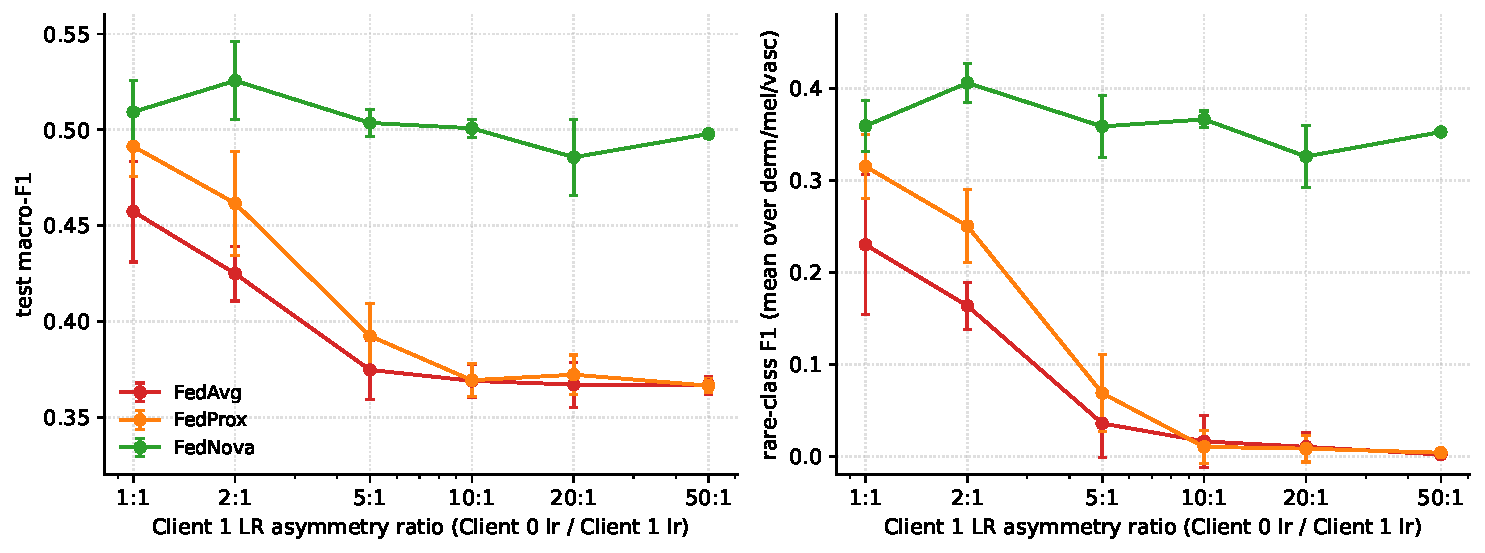
\includegraphics[width=\textwidth]{F_asymmetric_lr_L4.pdf}
\caption{Learning-rate asymmetry envelope at L4, $n=3$ per cell. Two panels:
test macro-F1 and rare-class F1 (mean over dermato, melanoma, vascular) vs
the Client 1 LR ratio on $\log_{10}$ axis from 1:1 to 50:1. FedAvg and
FedProx plateau at the rare-class floor; FedNova stays flat across the
envelope.}
\label{fig:lr-asymmetry-envelope}
\end{figure}


% =============================================================================
% Figure 5.6 placeholder -- heterogeneity escalation
% =============================================================================

\begin{figure}[h]
\centering
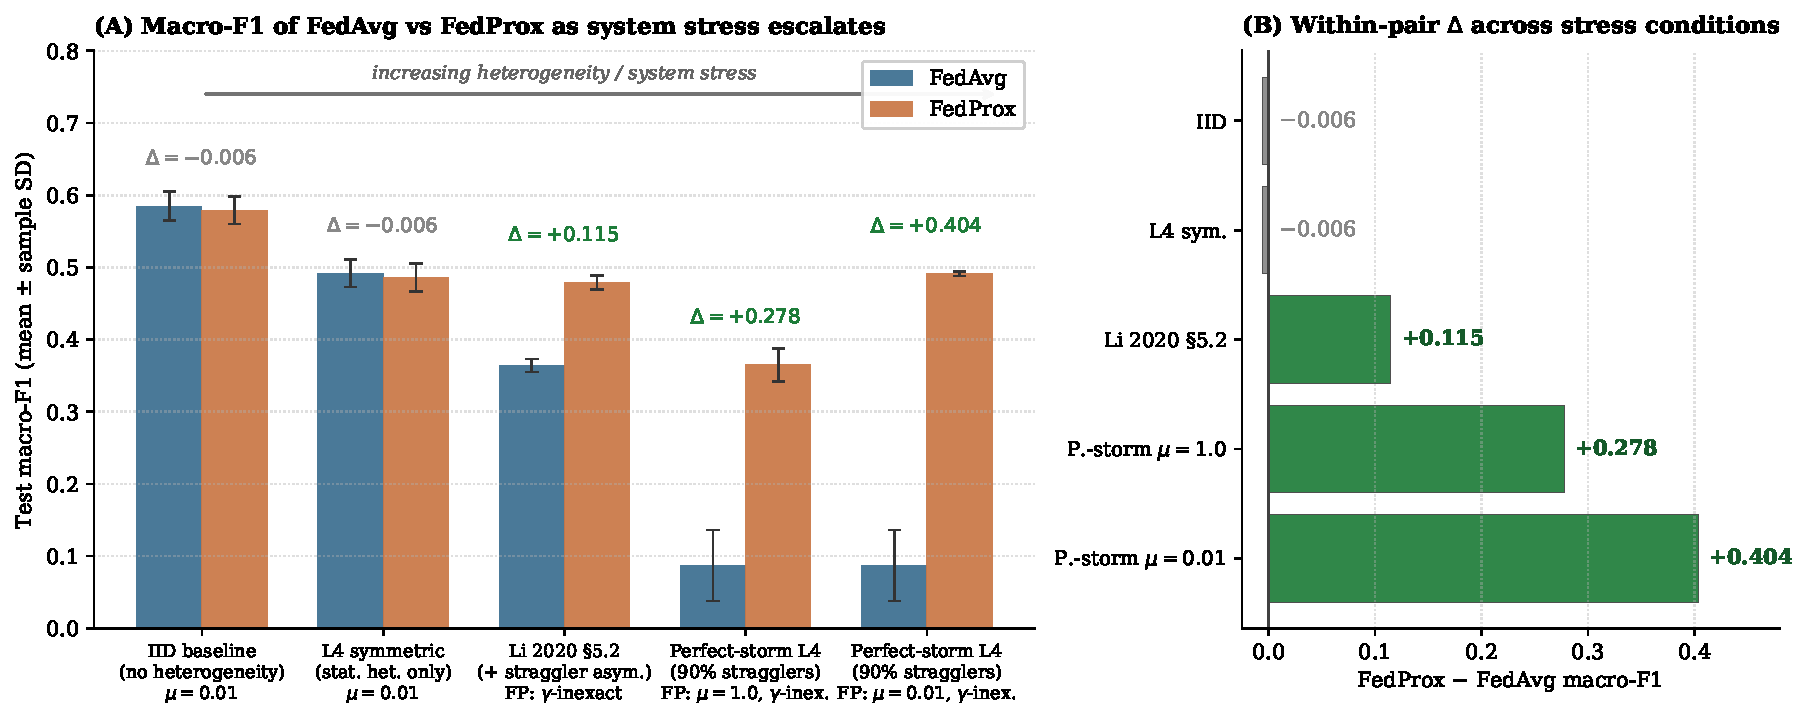
\includegraphics[width=0.85\textwidth]{F_heterogeneity_escalation.pdf}
\caption{Heterogeneity-escalation synthesis. Within-pair
$\Delta(\textrm{FedProx} - \textrm{FedAvg})$ macro-F1 across five regime cells
of increasing severity: IID Flower negative control ($-0.007$), symmetric L4
multi-seed node-pinned ($+0.005$), Li 2020 four-condition contrast
(FA+drop vs FP+$\gamma$-inex, $+0.115$), perfect-storm $\mu = 1.0$
($+0.278$), perfect-storm $\mu = 0.01$ ($+0.404$). The first two cells sit
inside seed noise; the last three are large, mechanism-isolable, and
regime-driven.}
\label{fig:heterogeneity-escalation}
\end{figure}



%%%%%%%%%%%%%%%%%%%%%%%%%%%%%%%%%%%%%%%%%%%%%%%%%%%%%%%%%%%%%%%%%%%%%%%%%%%%%%%
%% sec 5.6 -- Rare-class collapse into mel-nevi
%%%%%%%%%%%%%%%%%%%%%%%%%%%%%%%%%%%%%%%%%%%%%%%%%%%%%%%%%%%%%%%%%%%%%%%%%%%%%%%

% =============================================================================
% Results sec 5.6 -- Rare-class collapse + loss-side correction
% Compressed version. Target ~470 words.
% =============================================================================

\section{Rare-class collapse into mel-nevi, and why FedProx is not simply
an imbalance corrector}
\label{sec:rare-class-collapse}


\subsection*{\S\,5.6.1 Per-class collapse}

The low-macro-F1 cells in \S\S\,\ref{sec:li-straggler}--\ref{sec:lr-asymmetry}
fail the same way: rare-class images are routed to mel-nevi
(Figure~\ref{fig:cross-experiment-per-class}). Mean rare-to-mel-nevi
misrouting (over dermato, melanoma, vascular) ranges from $24\,\%$ in the
best protocol (perfect-storm FP $\mu = 0.01$, $n=3$) to $67\,\%$ in the
worst (perfect-storm FA+drop, $n=3$), and $28\,\%$ even under the IID
Flower negative control ($n=10$) --- a class-imbalance saturation that the
FL protocol preserves or amplifies but does not itself create.

The D1 5:1 cell isolates the optimiser dimension: melanoma per-class F1 is
$1.20\,\%$ for FedAvg, $6.13\,\%$ for FedProx, $46.34\,\%$ for FedNova
($n=3$ each) --- same disease, three detection regimes spanning two orders
of magnitude. Macro-F1 is structurally sensitive: each class enters with
weight $1/7$, so a single class dropping from per-class F1 $\approx 0.4$ to
$0.0$ moves macro by $\approx 0.057$, the order of the entire engineered
$\Delta$ in \S\,\ref{sec:statistical-heterogeneity}. The same
rare-class-concentration pattern reappears in the
\S\,\ref{sec:mu-sensitivity} $\mu = 1.0$ catastrophic cell
(Table~\ref{tab:mu-per-class}, where dermato loses $-0.101$, vascular
$-0.113$, and mel-nevi is invariant), so across three different mechanisms
--- aggregation dropout, learning-rate asymmetry, and over-regularisation
--- failure expresses itself in the same rare-class shape.

\begin{center}
\small
\begin{tabular}{p{0.16\linewidth} p{0.14\linewidth} c c c p{0.32\linewidth}}
\hline
Protocol                  & Algorithm & Rare-F1 & Melanoma F1 & Misrouting & Interpretation \\
\hline
Perfect-storm + drop      & FedAvg    & $0.000$ & $0.00\,\%$  & $67\,\%$   & Rare client dropped; flatline \\
Perfect-storm + $\gamma$  & FedProx ($\mu=0.01$) & $0.357$ & $38.27\,\%$ & $24\,\%$ & $\gamma$-inex preserves rare signal \\
D1 5:1 LR asymmetry       & FedAvg    & $0.036$ & $1.20\,\%$  & $51\,\%$   & Rare client under-weighted; gradual erosion \\
D1 5:1 LR asymmetry       & FedNova   & $0.359$ & $46.34\,\%$ & $26\,\%$   & $\tau$-normalisation preserves contribution \\
\hline
\end{tabular}
\end{center}

\noindent
These four cells span instant-collapse and gradual-erosion modes across
straggler and LR-asymmetry axes; the misrouting rate co-varies with rare-F1
across all four.


\subsection*{\S\,5.6.2 Collapse modes}

Two trajectories of the same failure mode. Perfect-storm FedAvg+drop's
validation trajectory flatlines at each seed's round-1 value for all 150
rounds (best-val checkpoint selected at round 1, untrained init beating
every trained checkpoint; across-seed mean test macro-F1 $= 0.087 \pm 0.049$):
the rare-class client is dropped every round, so its signal has no path
into the global parameters. D1 5:1 degrades gradually instead: the rare client's updates
are accepted but progressively under-weighted, macro-F1 drifts $0.457 \to
0.375$ with rare-F1 collapsing in lockstep. Instant collapse and gradual
erosion of the same rare-class-signal-suppression mechanism, distinguished
only by whether the rare-class updates are dropped wholesale or simply
under-weighted.


\subsection*{\S\,5.6.3 Loss-side imbalance correction: weighted CE and
focal loss}

To test whether the FedProx advantage might be class-imbalance correction
in disguise, we ran FedAvg and FedProx at L4 with three loss functions
($n=3$ per cell): plain cross-entropy, class-weighted CE with
inverse-frequency weights, and focal loss ($\gamma = 2$). Cells are test
macro-F1 $\pm$ SD with rare-class F1 in parentheses.

\begin{center}
\begin{tabular}{lccc}
\hline
Algorithm & CE & Weighted CE & Focal \\
\hline
FedAvg  & $0.477 \pm 0.002$ ($0.285$) & $\mathbf{0.505 \pm 0.023}$ ($\mathbf{0.367}$) & $0.467 \pm 0.002$ ($0.317$) \\
FedProx & $0.478 \pm 0.016$ ($0.291$) & $0.503 \pm 0.014$ ($0.346$)                   & $0.476 \pm 0.022$ ($0.304$) \\
\hline
\end{tabular}
\end{center}

Three observations. (i) Weighted CE is the strongest loss-side correction:
FedAvg+wCE $0.505$ marginally exceeds FedProx+CE $0.478$ in this L4
symmetric setting; the FedAvg-only CE-to-wCE intervention raises macro by
$+0.029$ and rare-F1 by $+0.082$. (ii) Focal helps rare-F1 ($+0.032$ on
FedAvg) but hurts macro ($-0.010$): focal trades macro for rare-recall,
while wCE wins on both at the tested $\gamma=2$ and inverse-frequency
weights. (iii) FedProx adds little on top of either: FP+wCE
$0.503 \pm 0.014$ sits inside FA+wCE's SD of $0.023$, and FP/FA differ by
$0.009$ at focal. FedProx is a drift/protocol intervention (per
\S\,\ref{sec:li-straggler}), not a substitute for direct loss-side
imbalance correction; the two axes can in principle be combined but are
tested only separately here ($n=3$, L4 symmetric only).

The \S\,\ref{sec:li-straggler} FedProx + $\gamma$-inexact result and this
\S\,5.6.3 weighted-CE result are not in tension: $\gamma$-inex restores
aggregation under straggler-induced signal loss, while weighted CE
re-weights rare classes during local training. They act at different
pipeline stages and address different failure modes (signal loss vs label
saturation); they could in principle be combined but are tested only
separately here.

The rare-class collapse documented here is clinically \emph{motivated},
not clinically \emph{validated}: DermaMNIST is a $28 \times 28$-pixel
benchmark and not a deployment artefact. The next section turns to the
per-round update-norm activity behind these per-class outcomes.


% =============================================================================
% Figure 5.7 placeholder
% =============================================================================

\begin{figure}[h]
\centering
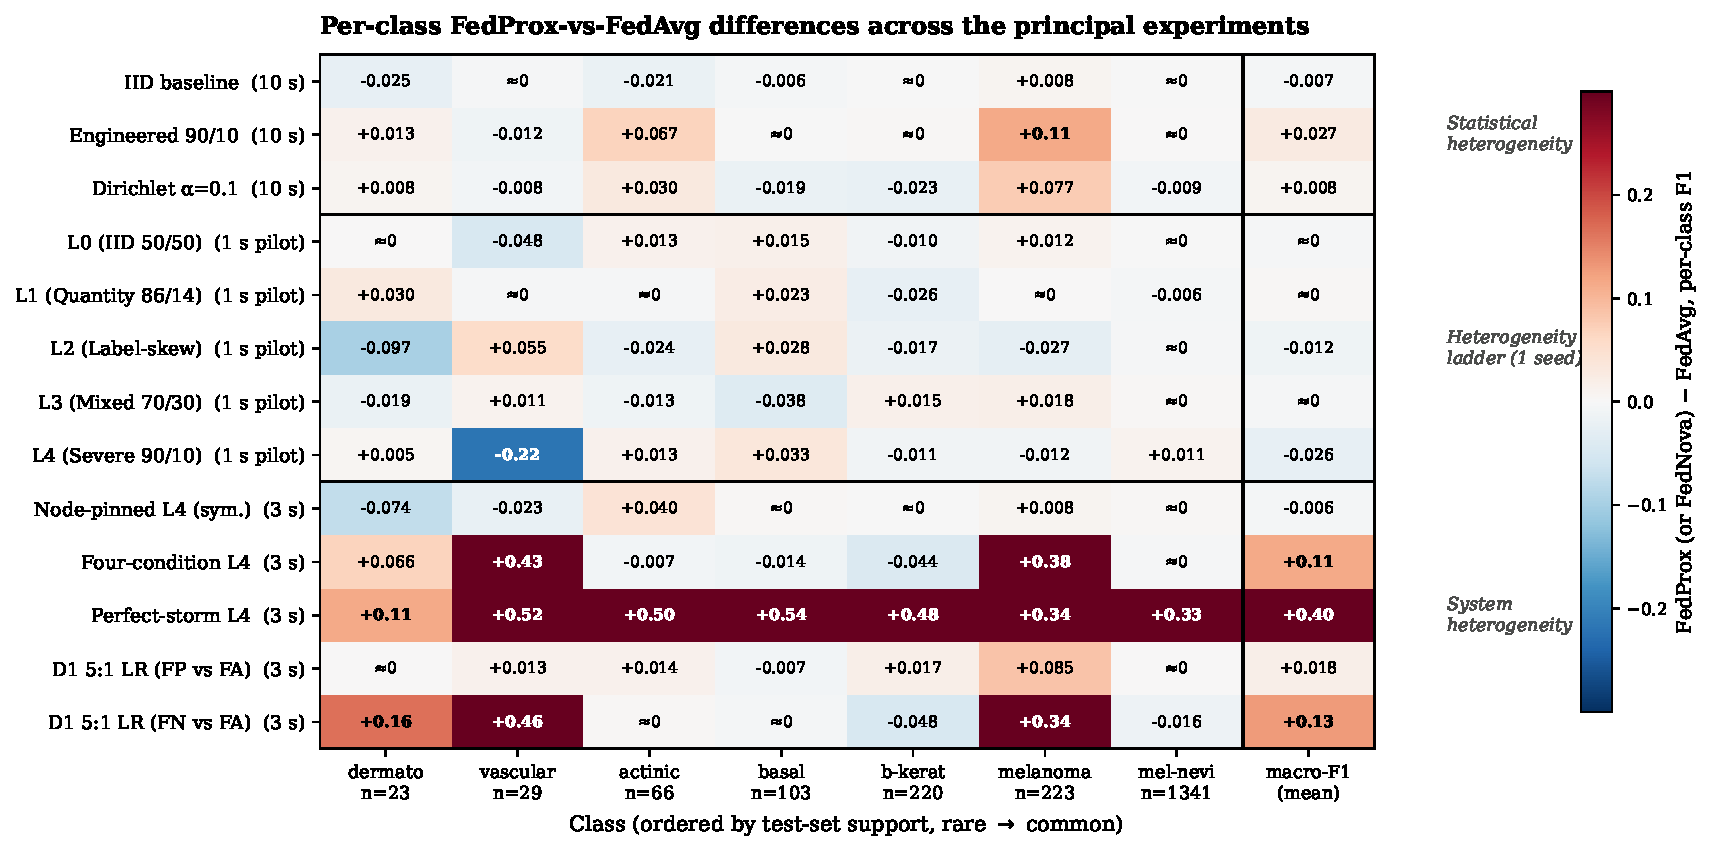
\includegraphics[width=\textwidth]{F_cross_experiment_per_class.pdf}
\caption{Per-class diagonal accuracy (correct-prediction rate per class)
across twelve protocol cells spanning baselines, Li 2020 straggler
conditions, perfect-storm, asymmetric LR (D1 1:1 and 5:1), and node-pinned
L4. The mel-nevi column saturates near $0.85$--$0.95$ in nearly every cell
while the dermato, melanoma, and vascular columns collapse to near zero in
the failing cells.}
\label{fig:cross-experiment-per-class}
\end{figure}



%%%%%%%%%%%%%%%%%%%%%%%%%%%%%%%%%%%%%%%%%%%%%%%%%%%%%%%%%%%%%%%%%%%%%%%%%%%%%%%
%% sec 5.7 -- Mechanism and robustness checks
%%%%%%%%%%%%%%%%%%%%%%%%%%%%%%%%%%%%%%%%%%%%%%%%%%%%%%%%%%%%%%%%%%%%%%%%%%%%%%%

% =============================================================================
% Results sec 5.7 -- Mechanism and robustness checks
% Compressed version. Target ~390 words.
% =============================================================================

\section{Mechanism and robustness checks}
\label{sec:mechanism-robustness}


\subsection*{\S\,5.7.1 Update-norm activity}

FedProx has two distinct mechanisms: a per-client proximal regulariser
that operates during local training, and a protocol-level $\gamma$-inexact
policy that operates at aggregation. The centrepiece
\S\,\ref{sec:li-straggler} result attributes the straggler-regime win to
the latter. The engineered update-norm reduction reported here reflects
the former: on the engineered partition ($n=10$), mean per-round
update-norm magnitude $\overline{\lVert \Delta w \rVert}$ is $1.523$ for
FedAvg vs $1.029$ for FedProx ($\mu = 0.01$) --- a $\approx 32\,\%$
reduction, consistent with the proximal term's drift-control intent. This
is a per-protocol observation of drift control under symmetric conditions,
distinct from the \S\,\ref{sec:li-straggler} aggregation-level mechanism
that carries the straggler-regime win.

Across 78 L4 runs pooled over eight algorithm-by-protocol cells (baselines,
Li 2020 four-condition, perfect-storm, asymmetric $\mu$, asymmetric LR,
weighted-CE), dominant-client mean update-norm magnitude correlates with
rare-class F1 at Spearman $r = +0.634$. The relative-influence ratio of the
rare-class-holding client (its update-norm $\div$ Client 0's) correlates
near zero across protocols, $r = -0.045$: it is not by itself predictive
when the comparison spans heterogeneous protocols.

Within the asymmetric-LR experiment alone ($n=27$ cells), the relative-
influence ratio does track rare-class F1 closely: $r = +0.80$ for FedAvg,
$r = +0.87$ for FedProx (cf.\ \S\,\ref{sec:lr-asymmetry}). Within-protocol
ordering does not extrapolate across the eight-cell L4 protocol family. We
report these correlations as exploratory mechanism evidence --- consistent
with a FedProx drift-control and a FedNova contribution-preservation
interpretation --- not as causal proof. The causal claim rests on
\S\,\ref{sec:li-straggler}.


\subsection*{\S\,5.7.2 Protocol-flip audit}

A protocol-flip audit across six multi-seed L4 cells under three
measurement choices (best-validation checkpoint, final-round, last-$K$-round
mean): large-effect cells (perfect-storm, Li 2020 asymmetric,
asymmetric-$\mu$) flip $0/9$ seed-level comparisons; small-effect cells
(node-pinned L4 s42, extended-rounds L3 s42, two-client 90/10 s456) flip
$3/9$. Small effects in symmetric protocols are reporting-protocol-fragile;
large asymmetric-protocol effects are not.

The chapter therefore weights conclusions by effect magnitude: the
\S\,\ref{sec:li-straggler} centrepiece ($+0.115$ macro-F1) and the
\S\,\ref{sec:lr-asymmetry} 50:1 FedNova--FedAvg gap ($+0.131$) are robust
to checkpoint choice; the sub-$1$\,pp differences in
\S\,\ref{sec:statistical-heterogeneity} are not. \S\,5.8 labels each
finding's strength accordingly.

The $B$-dissimilarity proxy, training-instability metric, asymmetric-$\mu$
Yao test, early-warning collapse detector, and small-hospital case study
are reported in Appendix~E as exploratory; none is load-bearing for any
\S\S\,5.2--5.8 conclusion.

These checks sketch a regime map for the three optimisers, summarised next.


% =============================================================================
% Figure 5.8 placeholder -- update-norm mechanism
% =============================================================================

\begin{figure}[h]
\centering
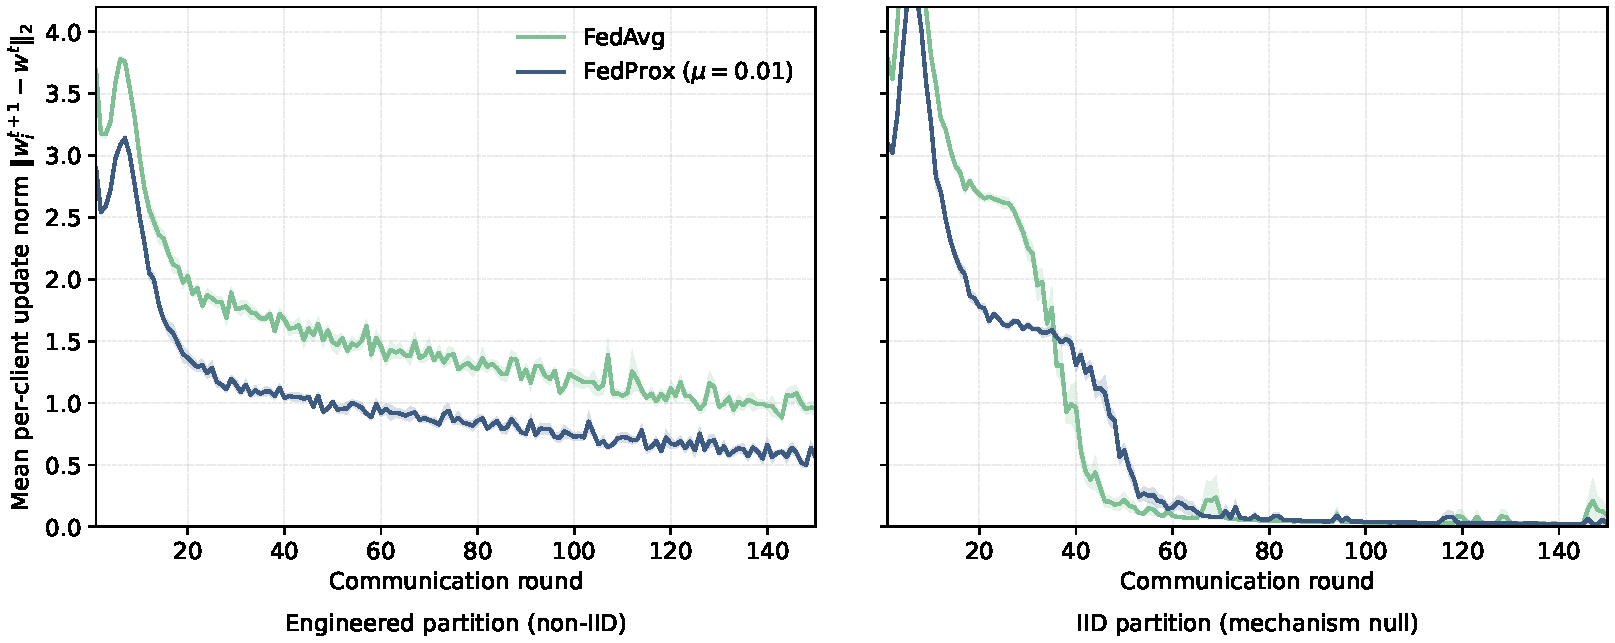
\includegraphics[width=0.85\textwidth]{F_update_norms.pdf}
\caption{Update-norm mechanism on the engineered partition. Mean per-round
$\lVert \Delta w \rVert$ trajectories per client for FedAvg vs FedProx
($n=10$ seeds); FedProx tracks lower throughout, consistent with the
proximal term's drift-control intent. Cross-protocol scatter panel
(78 L4 runs across 8 algorithm $\times$ protocol cells): Spearman
$r = +0.634$ between dominant-client mean update-norm and rare-class F1;
relative-influence ratio $r = -0.045$ across protocols.}
\label{fig:update-norms}
\end{figure}



%%%%%%%%%%%%%%%%%%%%%%%%%%%%%%%%%%%%%%%%%%%%%%%%%%%%%%%%%%%%%%%%%%%%%%%%%%%%%%%
%% sec 5.8 -- Integrated summary of findings
%%%%%%%%%%%%%%%%%%%%%%%%%%%%%%%%%%%%%%%%%%%%%%%%%%%%%%%%%%%%%%%%%%%%%%%%%%%%%%%

% =============================================================================
% Results sec 5.8 -- Integrated summary of findings
% Compressed. Target ~350 words. Closes with the central thesis sentence
% verbatim per guide sec 1.
% =============================================================================

\section{Integrated summary of findings}
\label{sec:integrated-summary}

Across the six experiments above, rare-class outcomes track rare-client
signal flow into the global model. FedAvg under stragglers drops the
rare-client update outright; FedProx with the proximal term alone does
not change which clients aggregate, so it cannot recover signal that was
discarded; FedProx + $\gamma$-inexact accepts partial rare-client updates
and recovers the signal; FedNova's $\tau$-normalisation rescales by
effective work and recovers signal under persistent LR asymmetry but
amplifies noise under random-$\tau$; weighted CE re-weights rare classes
during local training but only on clients that are actually aggregated.
The conditional thesis collapses to one rule: optimiser/protocol cells
preserve rare-class F1 if and only if rare-client signal reaches the
global model. Table~\ref{tab:final-claims} reports the chapter's findings
with explicit strength labels; five take-aways anchor the regime map.

(1) Statistical heterogeneity alone yields a small, runtime-sensitive
FedProx--FedAvg separation: Flower paired $\Delta = +0.007$ on the
engineered partition ($n=10$, 7/10 paired wins) with the pure-PyTorch
$\Delta = +0.027$ as the upper end of a $0.01$--$0.03$ band; the IID
negative control is $\Delta = -0.007$.

(2) The proximal coefficient is sharply tuned: the $\mu$-sweep traces an
inverted-$U$ with a useful single-decade range around $\mu = 0.01$ and a
catastrophic $\Delta = -0.074$ at $\mu = 1.0$ ($n=10$, 0/10 paired wins).

(3) Under Li-style straggler asymmetry at L4, the total FedProx--FedAvg gap
is $+0.115$ ($n=3$), but only $+0.004$ comes from the proximal term ---
about $96\,\%$ of the gain is mediated by $\gamma$-inexact partial-update
handling. The L1 cross-partition control flattens the $\gamma$-inexact
contribution to $+0.012$, confirming that the mechanism operates only when
the dropped client carries informationally unique class signal.

(4) FedNova is regime-dependent in both directions: the 50:1 FedNova--FedAvg
gap is $+0.131$ macro-F1 (the largest single-axis system-asymmetry gap in
the thesis, $n=3$), while random-$\tau$ straggler heterogeneity collapses
FedNova to mean macro-F1 $= 0.237$ with three of ten seeds reduced to the
majority-class-only baseline.

(5) Across failing protocols, the clinically motivated failure mode is
rare-class collapse into mel-nevi ($24\,\%$ to $67\,\%$ misrouting), and
weighted CE on FedAvg ($0.505$, $n=3$) matches or exceeds FedProx+CE
($0.478$, $n=3$) in the tested L4 symmetric setting --- FedProx is best
understood as a drift/protocol intervention rather than a class-imbalance
corrector.

Federated optimiser performance in imbalanced medical FL is regime-dependent:
FedAvg remains competitive under IID or symmetric low-risk protocols;
FedProx becomes valuable under Li-style straggler asymmetry mainly because
$\gamma$-inexact partial-update handling preserves the rare-client signal;
FedNova is robust under the tested learning-rate asymmetry but fails under
random-$\tau$ straggler regimes; and across failing settings, the common
clinical failure mode is rare-class collapse into the majority class
(mel-nevi). These results do not establish a universal ranking of FedAvg,
FedProx, and FedNova. They instead map which optimiser/protocol choices
preserve or lose rare-class performance under different heterogeneity
regimes.


% =============================================================================
% Table 5.5 -- Final claim-evidence-caveat summary
% =============================================================================

\begin{table}[h]
\centering
\small
\caption{Final claim--evidence--caveat summary. Strength labels: \emph{strong}
= multi-seed, mechanism-isolable, checkpoint-robust; \emph{medium} =
multi-seed but small effect or single-protocol; \emph{exploratory} =
correlational, single-protocol, or $n=3$ without mechanism isolation.}
\label{tab:final-claims}
\begin{tabular}{p{3.0cm}p{3.6cm}p{1.6cm}p{2.6cm}p{2.6cm}}
\hline
Claim & Evidence & Strength & Caveat & Implication \\
\hline
FedProx not free under IID & Flower IID $\Delta = -0.007$ ($n=10$) & strong & IID is artificial & Reach for FedProx only when heterogeneity exists \\
Stat-het alone gives fragile separation & Flower engineered $\Delta = +0.007$ (7/10 wins, $n=10$) & medium & Runtime-sensitive (PyTorch $+0.027$) & Do not recommend FedProx on partition alone \\
$\mu$ must be tuned & Sweep $n=10$: peak $+0.013$ at $\mu = 0.01$; $-0.074$ at $\mu = 1.0$ & strong & Engineered partition only & Default $\mu = 0.01$; do not raise under heterogeneity \\
$\gamma$-inexact dominates straggler gain & L4 four-condition $n=3$: total $+0.115$, $\gamma$-inex $+0.111$; L1 control $+0.012$ & strong & Simulated stragglers (epoch-count, not wall-clock) & Use FedProx + $\gamma$-inexact under straggler protocols \\
FedNova regime-dependent & LR envelope: FN holds $0.49$--$0.53$ across 1:1--50:1 ($n=3$); random-$\tau$ collapses to $0.237$ ($n=10$, 3/10 majority) & medium--strong & Wang 2020 stable-$\tau$ assumption violated by random-$\tau$ & Prefer FedNova under persistent LR asymmetry, not under random-$\tau$ \\
Rare-class collapse is the clinical failure mode & Misrouting $24\,\%$--$67\,\%$; D1 5:1 melanoma F1 $= 1.2$/$6.1$/$46.3\,\%$ ($n=3$) & strong & Single dataset, $28 \times 28$ resolution & Report per-class metrics; macro-F1 alone hides it \\
wCE competes with FedProx & L4 $n=3$: FA+wCE $0.505$ vs FP+CE $0.478$ & medium & $n=3$, L4 symmetric only & Loss-side rebalancing is a competitive intervention \\
Update-norms support drift-control reading & Engineered: FA $1.523$ vs FP $1.029$ ($-32\,\%$); cross-protocol $r = +0.634$ & exploratory & Within-protocol $r$ does not extrapolate & Drift-control reading is supported, not proven \\
\hline
\end{tabular}
\end{table}



%%%%%%%%%%%%%%%%%%%%%%%%%%%%%%%%%%%%%%%%%%%%%%%%%%%%%%%%%%%%%%%%%%%%%%%%%%%%%%%
%% sec 5.9 -- Limitations
%%%%%%%%%%%%%%%%%%%%%%%%%%%%%%%%%%%%%%%%%%%%%%%%%%%%%%%%%%%%%%%%%%%%%%%%%%%%%%%

% =============================================================================
% Results sec 5.9 -- Limitations
% Compressed. Target ~200 words. One-line bullets, terse.
% =============================================================================

\section{Limitations}
\label{sec:limitations}

\begin{itemize}
\setlength\itemsep{0.15em}
\item Single dataset at low resolution (DermaMNIST $28 \times 28$); no
replication on Camelyon, full-resolution ISIC, or non-dermatology MedMNIST
subsets.
\item Mixed federation sizes: 7-client for the engineered headline and
statistical-heterogeneity settings; 2-client for the mechanism probes
(Li 2020 four-condition, perfect-storm, asymmetric LR, weighted-CE,
asymmetric $\mu$, node-pinned L4). No cross-scale generalisation claim is
made between the two sizes.
\item Local-epoch budget fixed at $E = 20$; straggler protocols are
simulated via local-epoch counts rather than wall-clock deadlines.
\item $n = 3$ paired seeds for several strong asymmetry claims
(Li 2020 four-condition, perfect-storm, asymmetric LR, weighted-CE,
asymmetric $\mu$). No significance test is applied at this sample size.
\item The heterogeneity ladder is a single-seed pilot and is reported as
such; multi-seed promotion exists only at L4 ($n = 3$).
\item Runtime divergence between pure-PyTorch ($+0.027$) and Flower
($+0.007$) on the engineered partition limits magnitude claims; only
direction is robust across runtimes.
\item No SCAFFOLD, FedAdam, or FedYogi comparator; the optimiser space is
FedAvg, FedProx, FedNova only.
\item No AUC or calibration metrics; predictions are argmax only.
\item Per-client validation distributions were not logged centrally;
q-FFL-style fairness CDFs and Sheller-style cross-client generalisation
grids cannot be produced from existing artefacts.
\end{itemize}


%% =============================================================================
%% END OF RESULTS BODY
%% =============================================================================

\end{document}
